\documentclass[10pt, letterpaper]{article}
\usepackage[vmargin=1in, hmargin=1in]{geometry}
\usepackage{fancyhdr, setspace, inconsolata, xcolor, sectsty, epstopdf, listings, siunitx, longtable, csvsimple}
\usepackage{graphicx, float, amsfonts, amsmath, epstopdf, hyperref, soul, hyperref, caption, makecell}
\usepackage{pdfpages}
\usepackage[title]{appendix}
\sisetup{output-exponent-marker=\ensuremath{\mathrm{E}}}
\DeclareSIUnit{\decade}{\text{dec}}

% ------------------------------------
% DEFINE PAGE HEADERS AND FOOTERS HERE
% ------------------------------------
\pagestyle{fancy}
\rhead{\textit{Final MATLAB Project}}
\lhead{\textit{ECE 580 Small Satellite Design}}
\lfoot{\textit{S. Ribeiro \& R. Yerrabelli}}
\rfoot{\textit{Page \thepage}}
\cfoot{}

%------------------------------
% DEFINE CODE HIGHLIGHTING RULES
%------------------------------

\definecolor{dkgreen}{rgb}{0,0.6,0}
\definecolor{gray}{rgb}{0.5,0.5,0.5}
\definecolor{brightmaroon}{rgb}{0.76, 0.13, 0.28}

 \lstset{language=Matlab,
   keywords={break,case,catch,continue,else, elseif, end, for, function,
      global,if,otherwise,persistent,return,switch,try,while},
   basicstyle=\ttfamily\fontseries{lc},
   keywordstyle=\color{blue},
   commentstyle=\color{dkgreen},
   stringstyle=\color{brightmaroon},
   numbers=left,
   numberstyle=\small\color{gray},
   stepnumber=1,
   numbersep=10pt,
   backgroundcolor=\color{white},
   tabsize=4,
   showspaces=false,
   showstringspaces=true,
   breaklines = true
   }
   
 \lstset{framexleftmargin=8mm, frame=shadowbox, rulesepcolor=\color{gray}}
% -------------------------
% DEFINE SECTION STYLE HERE
% -------------------------
\sectionfont{\sffamily}
\subsectionfont{\sffamily}
\subsubsectionfont{\sffamily}


% -------------------------
% DEFINE CAPTION STYLE HERE
% -------------------------
\captionsetup{font={small,stretch=1}}

\title{\sffamily{Mathematical Model of a CubeSat Attitude Determination System in MATLAB}}
\author{\sffamily{Sergio Ribeiro, Rohith Yerrabelli}}
\date{\sffamily{Tuesday May 3, 2022}}

% ----------------------------
% DEFINE DOCUMENT STRETCH HERE
% ----------------------------
\newcommand\docstretch{1.2}

\begin{document}
\maketitle

\begin{figure}[H]
	\centering
	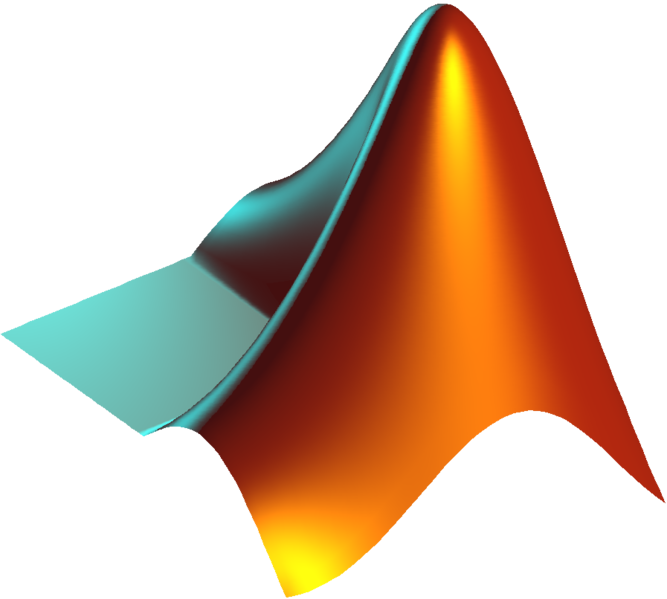
\includegraphics[scale=0.5]{Matlab_Logo.png}
\end{figure}

\setstretch{\docstretch}
\newpage
\section{Project Purpose}

The purpose of this project is to provide a mathematical model for computing a CubeSat's orientation based on the response of six photo-diodes on the center of each face of the cube. The first part of this project is to provide a mathematical description of light falling on the face of each cube.

We will need to come up with three things,

\begin{enumerate}
    \item A method to describe the orientation of the CubeSat in three dimensional space
    \item A method to compute and define cube rotations
    \item A method to compute the light falling on a cube face based on the cube rotation
\end{enumerate}

Once these items are properly described, we can then begin to work backwards and compute the diode responses on each cube face. Here are some simplifying assumptions we are making about this problem,

\begin{enumerate}
    \item We are assuming that the diode response is linear and proportional to the light falling on it. We do not consider the case of where the photo-diode is saturated or pushed to a non-linear region of the curve.
    \item We are not considering the effect of temperature on the diode response curve. This would be proportional to the light falling on the diode as this will heat up the panel the diode rests on.
    \item We are not considering the reflection of the light source falling on the other faces of the cube.
    \item We assume the light source is at a nearly infinite distance, so the light flux can be assumed to be constant in the vicinity of the space of the CubeSat.
\end{enumerate}

\subsection{Describing the CubeSat Orientation}

In Figure \ref{fig:OriginalCubeSat} we can see the CubeSat described by a series of six vectors. Each of the vectors are unit vectors are orthogonal to each other. Each of the unit vectors is normal to the plane of the face it describes.

We will use the following naming convention for each of the faces that are described by the unit vectors,

\begin{center}
\begin{tabular}{|c|c|c|}
    \hline
    Face Name & Unit Vector Associated & Vector Notation \\ \hline
    North X & $+\mathbf{\hat{x}}$ & $\langle +1, 0, 0 \rangle$ \\
    North Y & $+\mathbf{\hat{y}}$ & $\langle 0, +1, 0 \rangle$ \\
    North Z & $+\mathbf{\hat{z}}$ & $\langle 0, 0, +1 \rangle$ \\
    South X & $-\mathbf{\hat{x}}$ & $\langle -1, 0, 0 \rangle$ \\
    South Y & $-\mathbf{\hat{y}}$ & $\langle 0, -1, 0 \rangle$ \\
    South Z & $-\mathbf{\hat{z}}$ & $\langle 0, 0, -1 \rangle$ \\ \hline
\end{tabular}
\end{center}

\begin{figure}[H]
	\centering
	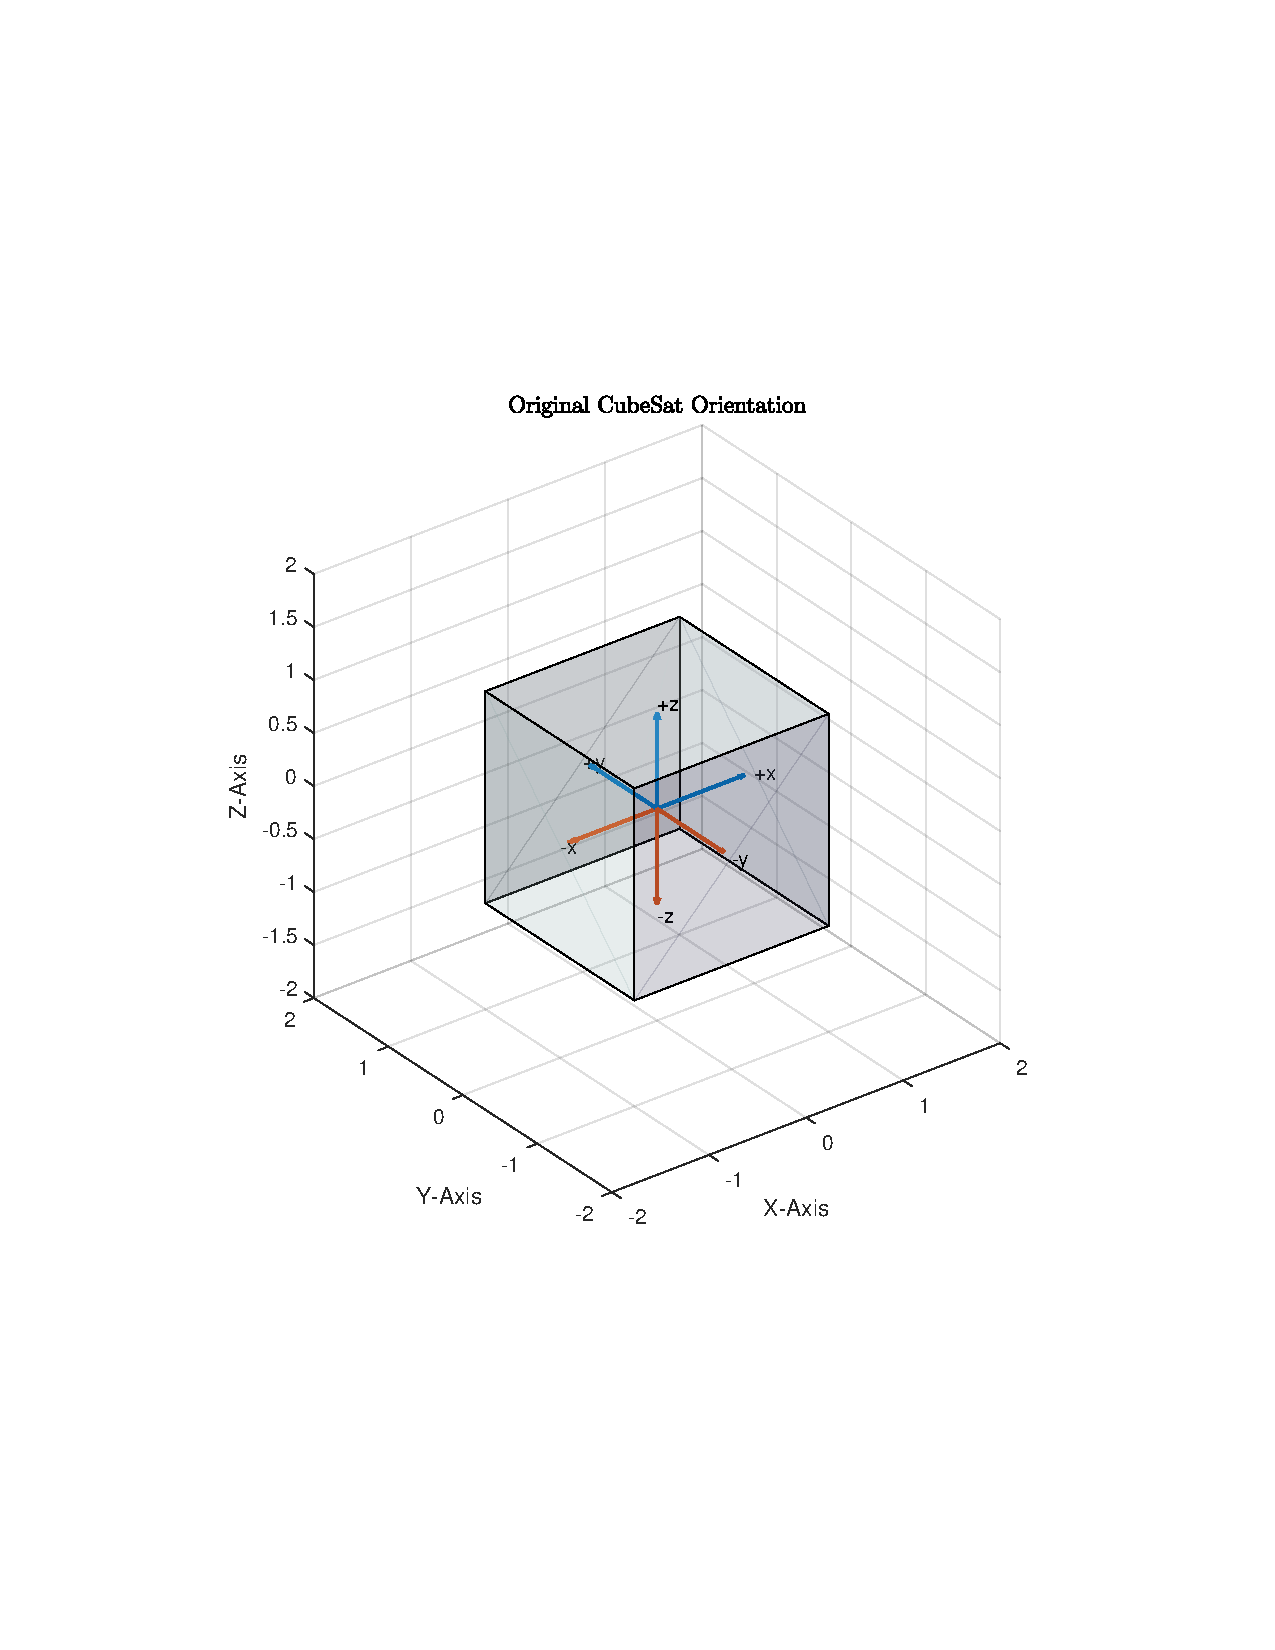
\includegraphics[scale=0.8]{OriginalCubeSat.pdf}
    \caption{The CubeSat in an orientation where all the faces are aligned with the $x$, $y$ and $z$ axes.}
    \label{fig:OriginalCubeSat}
\end{figure}

\subsection{Computing CubeSat Rotation in 3D Space}

Computing roll, pitch and yaw coordinates can be achieved using three rotation matrices as defined below. The $R_{x}$ matrix defines `roll', the $R_{y}$ matrix defines `pitch' and the $R_{z}$ matrix defines `yaw'.


\[
  R_{x}(\theta)=
  \left( {\begin{array}{ccc}
   \cos{\theta} & -\sin{\theta} & 0 \\
   \sin{\theta} & \cos{\theta} & 0 \\
   0 & 0 & 1
  \end{array} } \right)
\]

\[
  R_{y}(\theta)=
  \left( {\begin{array}{ccc}
   \cos{\theta} & 0 & \sin{\theta} \\
   0 & 1 & 0 \\
   -\sin{\theta} & 0 & \cos{\theta}
  \end{array} } \right)
\]

\[
  R_{z}(\theta)=
  \left( {\begin{array}{ccc}
   1 & 0 & 0 \\
   0 & \cos{\theta} & -\sin{\theta} \\
   0 & \sin{\theta} & \cos{\theta}
  \end{array} } \right)
\]

Multiplying a column vector (as shown below),

\[
  \left( {\begin{array}{c}
   r_{x}  \\
    r_{y} \\
   r_{z} 
  \end{array} } \right)
\]

By $R_{x}$, $R_{y}$ and $R_{z}$ will rotate the vector by roll, pitch and yaw in the order they are multiplied. For our sake we will define our rotations in terms of roll, pitch and yaw in that order.

Therefore our overall rotation matrix will be,
\begin{equation*}
R(\alpha, \beta, \gamma) = R_{x}(\alpha) \cdot R_{y}(\beta) \cdot R_{z}(\gamma)
\end{equation*}

Figure \ref{fig:RotatedCubeSat} shows how the rotation matrices rotate the entire orientation of the cube and the vectors describing each cube face are rotated with it.

\begin{figure}[H]
	\centering
	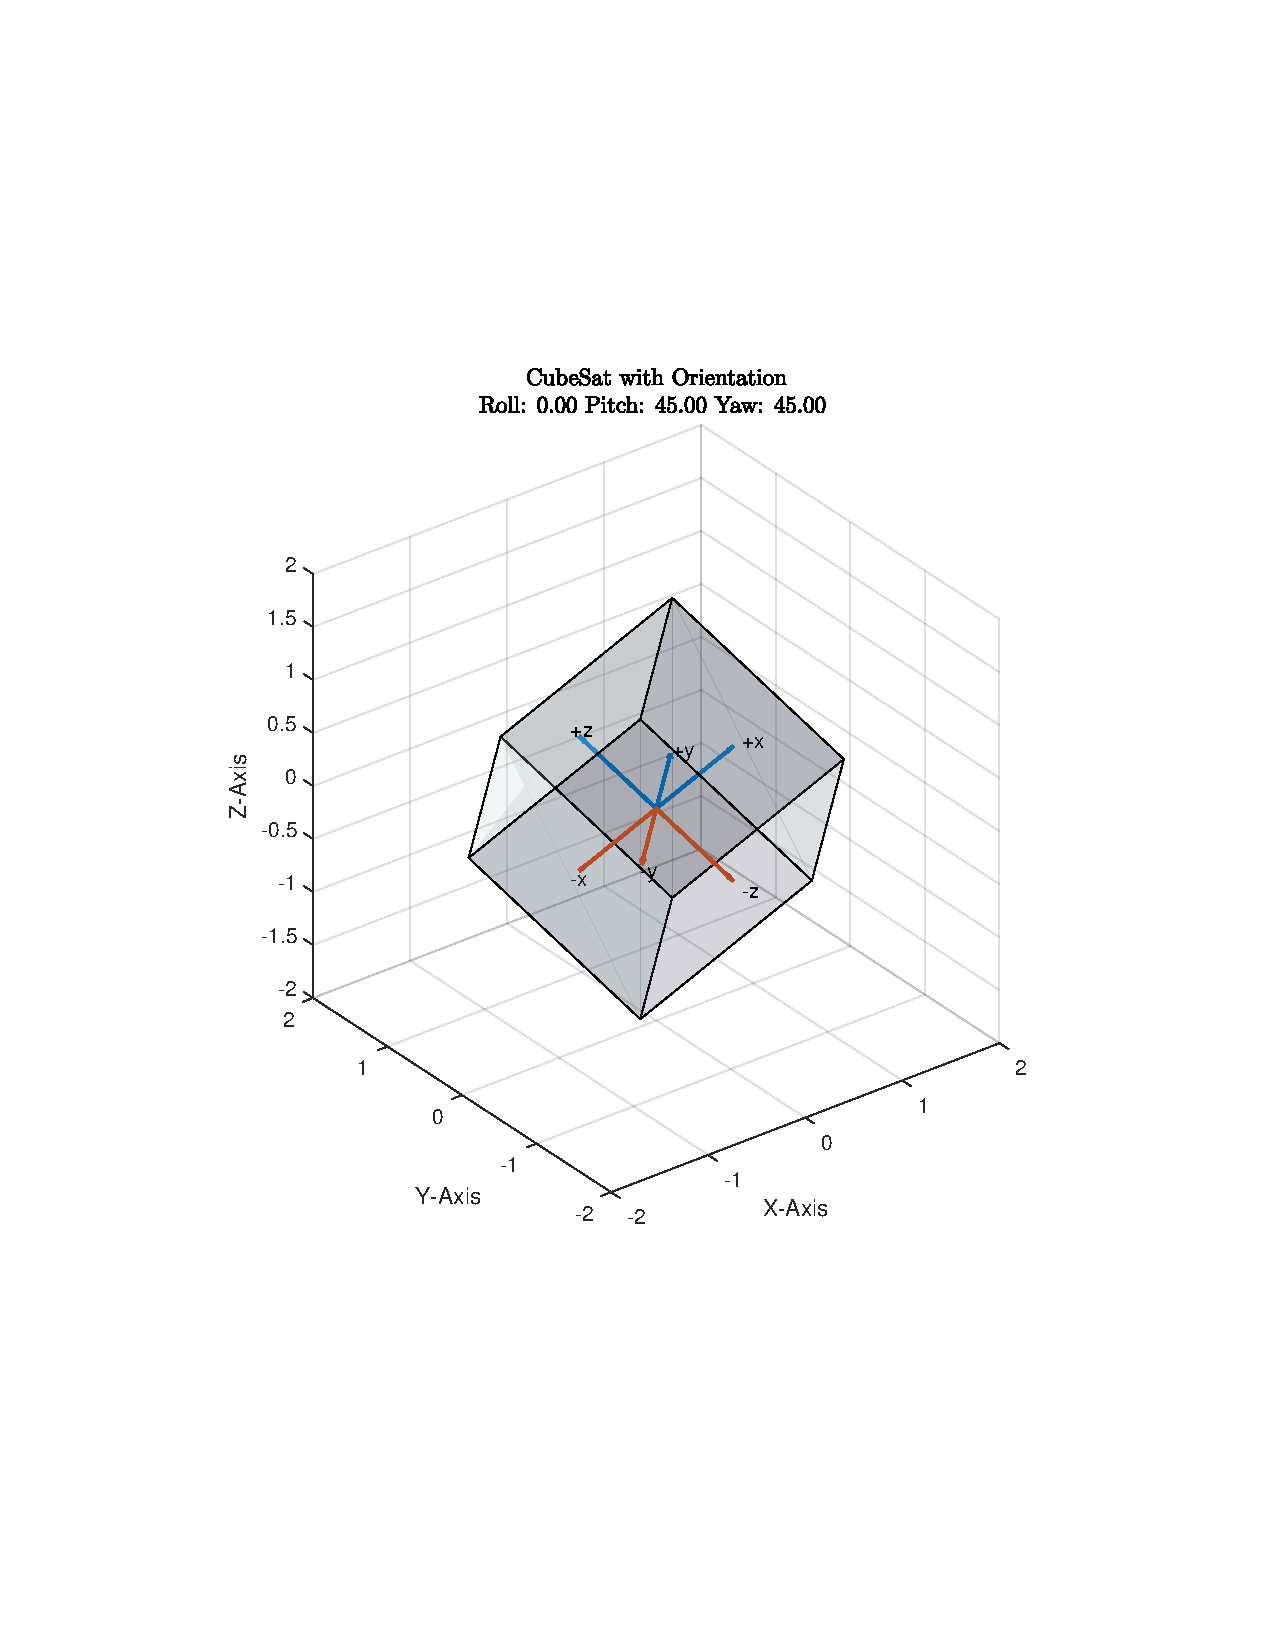
\includegraphics[scale=0.8]{RotatedCubeSat.pdf}
    \caption{The CubeSat has been rotated with a roll of $0^{\circ}$, a pitch of $45^{\circ}$ and a yaw of $45^{\circ}$. }
    \label{fig:RotatedCubeSat}
\end{figure}

\subsection{Computing the Light Flux}

Computing the light flux can be accomplished by defining what the light field looks like in the vicinity of the cube. The light flux is assumed to be from the sun and since the light source is far (infinite distance) the light flux is a constant vector field.

We will define this vector field as,

\begin{align*}
    \mathbf{\Phi}_{\text{Sun}}(x, y, z) &= \phi_{x} \cdot \mathbf{\hat{x}} + \phi_{y} \cdot \mathbf{\hat{y}} + \phi_{z} \cdot \mathbf{\hat{z}} \\
    &= \langle \phi_{x}, \phi_{y}, \phi_{z} \rangle
\end{align*}

This shows that it is a constant vector throughout the entire three dimensional space we are considering. Now computing the light flux through each space will be a simple task. Ordinarily we would need to compute a surface integral for each surface, however since each surface is perfectly flat and square and the vector field is constant, no calculus is required to evaluate the light flux through each face.

The light flux is a scalar quantity that can be calculated by the following equations where $A$ is the area of the cube face,

\begin{align*}
    \Phi_{\text{North, x}} &= -A \cdot \mathbf{\Phi}_{\text{Sun}}(x, y, z) \cdot \mathbf{\hat{x}}_\text{North} \\
    \Phi_{\text{North, y}} &= -A \cdot \mathbf{\Phi}_{\text{Sun}}(x, y, z) \cdot \mathbf{\hat{y}}_\text{North} \\
    \Phi_{\text{North, z}} &= -A \cdot \mathbf{\Phi}_{\text{Sun}}(x, y, z) \cdot \mathbf{\hat{z}}_\text{North} \\
    \Phi_{\text{South, x}} &= -A \cdot \mathbf{\Phi}_{\text{Sun}}(x, y, z) \cdot \mathbf{\hat{x}}_\text{South} \\
    \Phi_{\text{South, y}} &= -A \cdot \mathbf{\Phi}_{\text{Sun}}(x, y, z) \cdot \mathbf{\hat{y}}_\text{South} \\
    \Phi_{\text{South, z}} &= -A \cdot \mathbf{\Phi}_{\text{Sun}}(x, y, z) \cdot \mathbf{\hat{z}}_\text{South} \\
\end{align*}

When using these formulas, the positive flux numbers represent cubes that are directly in the light. The negative numbers are faces that are shaded. The response of the photodiodes of the negative numbers would be zero in reality.

\section{Sample Data Generated for Diodes}

The sample data generated from a known sun flux vector field $\mathbf{\Phi}_{\text{Sun}}(x, y, z)$ and known cube orientation specified by roll, pitch and yaw angles are are recorded in CSV files. They have been attached to the project as raw files to look at.

The CSV files are \texttt{RollAngleChange.csv}, \texttt{PitchAngleChange.csv} and \texttt{YawAngleChange.csv}. The following plots will show the diode response curves associated with changing roll, pitch and yaw angles. The starting sun flux vector is $\langle 15, 18, 12 \rangle$. The default satellite orientation is $0^{\circ}$ roll, $0^{\circ}$ pitch and $0^{\circ}$ yaw. Then each of these parameters is stepped from $0^{\circ}$ to $90^{\circ}$. The diode response curves are plotted in Figures \ref{fig:RollAngleChange}, \ref{fig:PitchAngleChange} and \ref{fig:YawAngleChange}.

\begin{figure}[H]
	\centering
	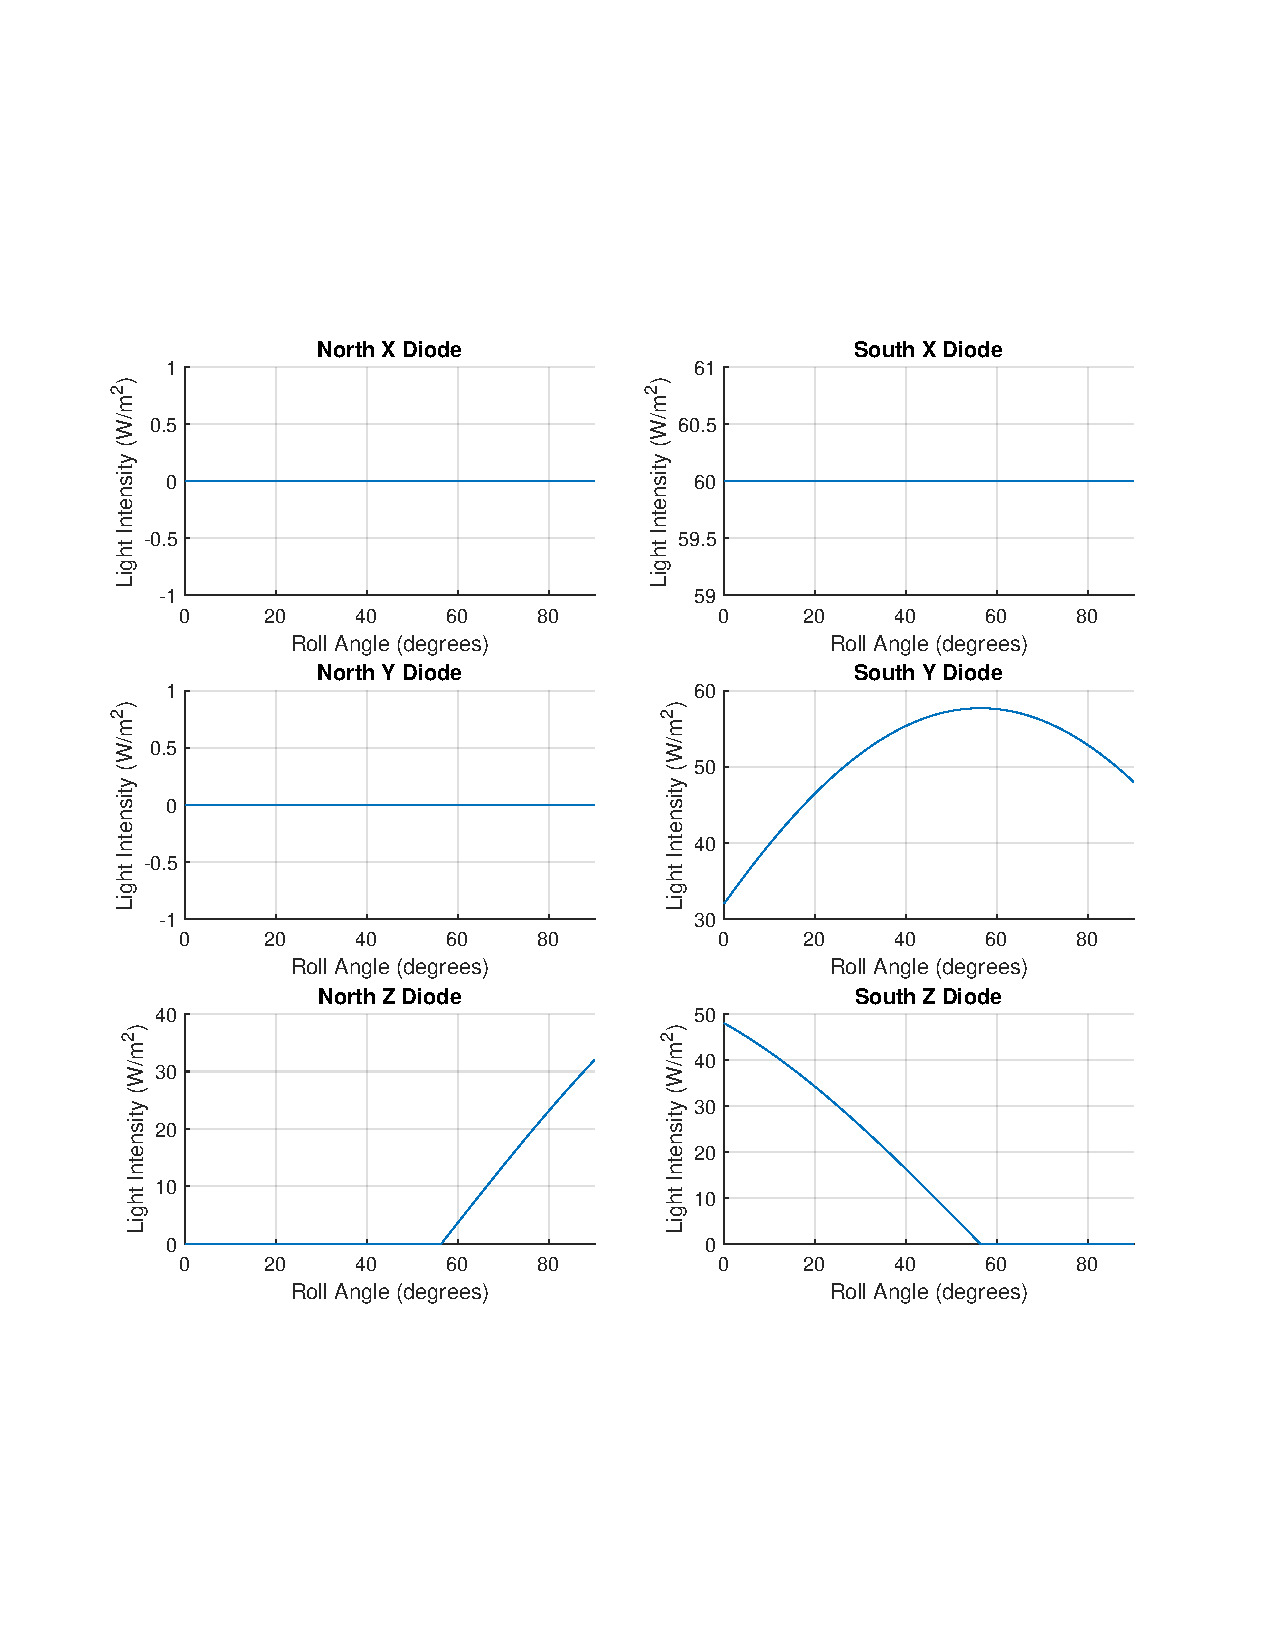
\includegraphics[scale=0.8]{RollAngle_DiodeResponse.pdf}
    \caption{Roll angle is changed continuously from $0^{\circ}$ to $90^{\circ}$.}
    \label{fig:RollAngleChange}
\end{figure}

\begin{figure}[H]
	\centering
	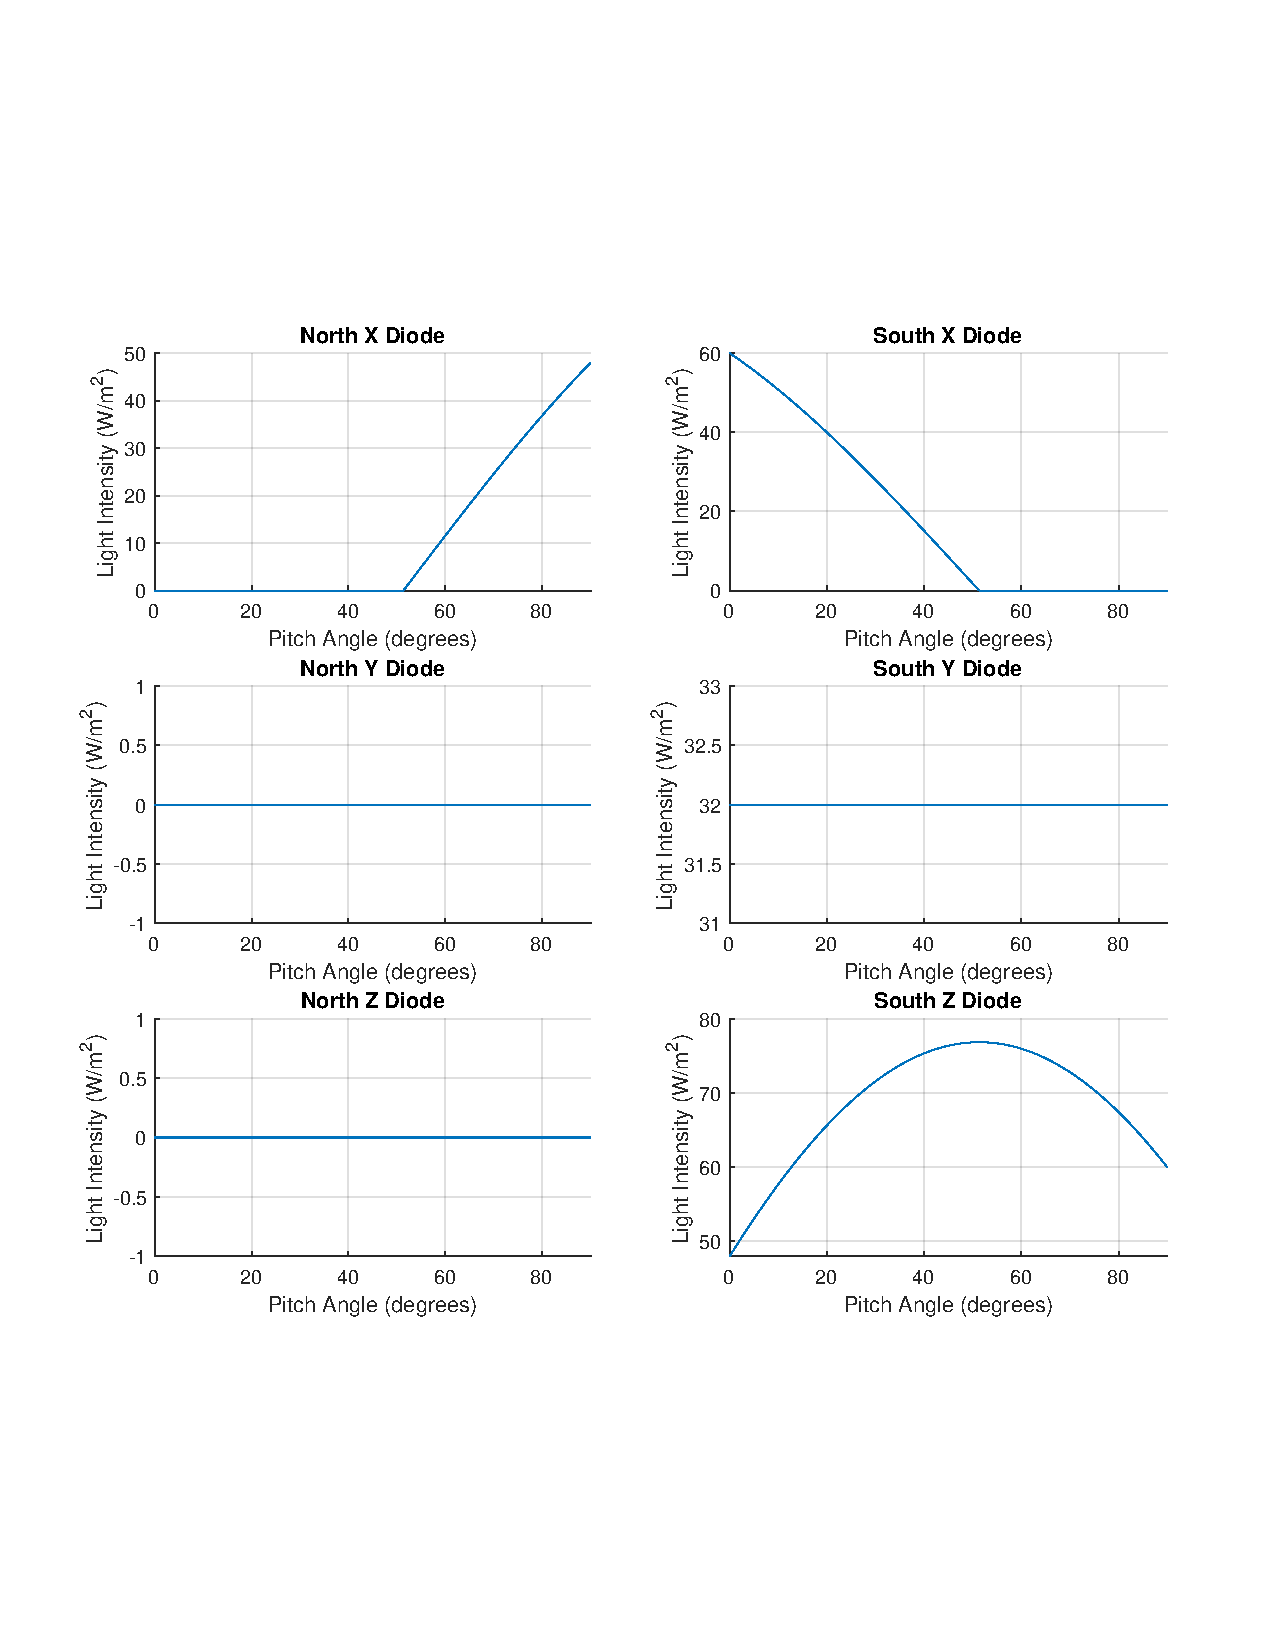
\includegraphics[scale=0.8]{PitchAngle_DiodeResponse.pdf}
    \caption{Pitch angle is changed continuously from $0^{\circ}$ to $90^{\circ}$.}
    \label{fig:PitchAngleChange}
\end{figure}

\begin{figure}[H]
	\centering
	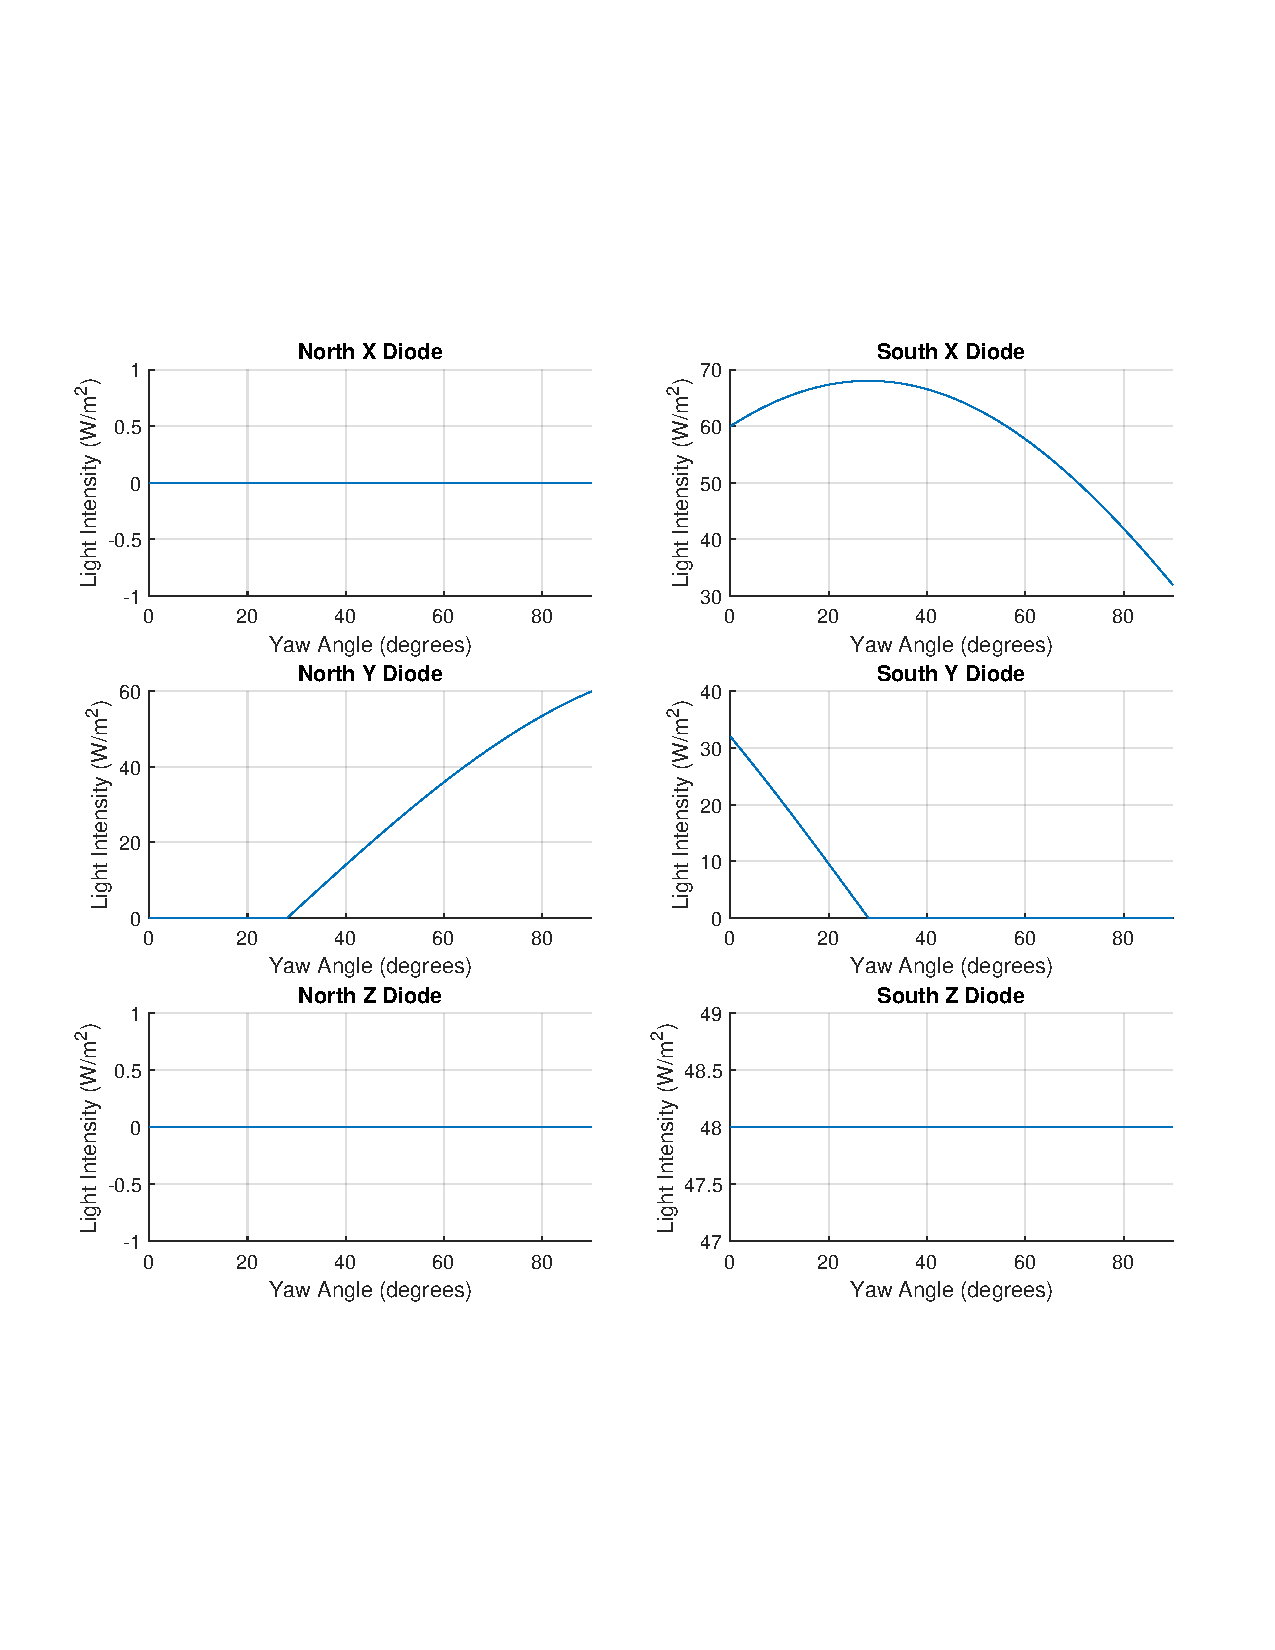
\includegraphics[scale=0.8]{YawAngle_DiodeResponse.pdf}
    \caption{Yaw angle is changed continuously from $0^{\circ}$ to $90^{\circ}$.}
    \label{fig:YawAngleChange}
\end{figure}


\section{Determining CubeSat Orientation from Diode Response}

\subsection{Octant Naming Convention}
From our proposed model of how the light flux shines on each face of the CubeSat, we can see that any given orientation only illuminates three cube faces at any given moment. Knowing this information allows us to at least know what octant the cube is oriented and where the light is shining. It also tells us approximately what octant the source is in. Octants will be named according to which corners of the unit cube are present in the octant. Each corner is specified by the unit vector sum associated with each cube corner.

\begin{table}[H]
\centering
    \begin{tabular}{|c|c|c|}
    \hline
    Octant Name & Corresponding Vector & Decimal \\ \hline
    000 & $\langle -1,-1,-1 \rangle$ & 0 \\
    001 & $\langle -1,-1,+1 \rangle$ & 1 \\
    010 & $\langle -1,+1,-1 \rangle$ & 2 \\
    011 & $\langle -1,+1,+1 \rangle$ & 3 \\
    100 & $\langle +1,-1,-1 \rangle$ & 4 \\
    101 & $\langle +1,-1,+1 \rangle$ & 5 \\
    110 & $\langle +1,+1,-1 \rangle$ & 6 \\
    111 & $\langle +1,+1,+1 \rangle$ & 7 \\ \hline
    \end{tabular}
    \label{table:OctantNamingConvention}
    \caption{Octant naming convention based on vectors.}
\end{table}

\subsection{Insolubility of the Rotation Matrix by Direct Means}
Attempting to solve the attitude control problem directly without making some simplifying assumptions yields a set of difficult equations to solve that we have not found any easy solutions to.

Fundamentally the equations that we need to solve are the following,

\begin{align*}
    \Phi_{\text{North, x}} &= -A \cdot \mathbf{\Phi}_{\text{Sun}}(x, y, z) \cdot R(\alpha, \beta, \gamma) \mathbf{\hat{x}} \\
    \Phi_{\text{North, y}} &= -A \cdot \mathbf{\Phi}_{\text{Sun}}(x, y, z) \cdot R(\alpha, \beta, \gamma) \mathbf{\hat{y}} \\
    \Phi_{\text{North, z}} &= -A \cdot \mathbf{\Phi}_{\text{Sun}}(x, y, z) \cdot R(\alpha, \beta, \gamma) \mathbf{\hat{z}} \\
    \Phi_{\text{South, x}} &= A \cdot \mathbf{\Phi}_{\text{Sun}}(x, y, z) \cdot R(\alpha, \beta, \gamma) \mathbf{\hat{x}} \\
    \Phi_{\text{South, y}} &= A \cdot \mathbf{\Phi}_{\text{Sun}}(x, y, z) \cdot R(\alpha, \beta, \gamma) \mathbf{\hat{y}} \\
    \Phi_{\text{South, z}} &= A \cdot \mathbf{\Phi}_{\text{Sun}}(x, y, z) \cdot R(\alpha, \beta, \gamma) \mathbf{\hat{z}} \\
\end{align*}

In the set of above equations the quantities of flux on each cube face is known as that is what the diodes measure, the area of each cube face ($A$) is known and the unit vector values $\mathbf{\hat{x}}$, $\mathbf{\hat{y}}$ and $\mathbf{\hat{z}}$ are known. What we are trying to solve for is $R$. If we treat all the quantities as matrices our equations become,

\[
\begin{bmatrix}
\Phi_{\text{North, x}} \\
\Phi_{\text{North, y}} \\
\Phi_{\text{North, z}}
\end{bmatrix}
= -A
\begin{bmatrix}
\Phi_{\text{Sun, x}} & \Phi_{\text{Sun, y}} & \Phi_{\text{Sun, z}} \\
\Phi_{\text{Sun, x}} & \Phi_{\text{Sun, y}} & \Phi_{\text{Sun, z}} \\
\Phi_{\text{Sun, x}} & \Phi_{\text{Sun, y}} & \Phi_{\text{Sun, z}} \\
\end{bmatrix}
\begin{bmatrix}
R_{11} & R_{12} & R_{13} \\
R_{21} & R_{22} & R_{23} \\
R_{31} & R_{32} & R_{33}
\end{bmatrix}
\begin{bmatrix}
1 & 0 & 0 \\
0 & 1 & 0 \\
0 & 0 & 1 \\
\end{bmatrix}
\]

and,

\[
\begin{bmatrix}
\Phi_{\text{South, x}} \\
\Phi_{\text{South, y}} \\
\Phi_{\text{South, z}}
\end{bmatrix}
= -A
\begin{bmatrix}
\Phi_{\text{Sun, x}} & \Phi_{\text{Sun, y}} & \Phi_{\text{Sun, z}} \\
\Phi_{\text{Sun, x}} & \Phi_{\text{Sun, y}} & \Phi_{\text{Sun, z}} \\
\Phi_{\text{Sun, x}} & \Phi_{\text{Sun, y}} & \Phi_{\text{Sun, z}} \\
\end{bmatrix}
\begin{bmatrix}
R_{11} & R_{12} & R_{13} \\
R_{21} & R_{22} & R_{23} \\
R_{31} & R_{32} & R_{33}
\end{bmatrix}
\begin{bmatrix}
-1 & 0 & 0 \\
0 & -1 & 0 \\
0 & 0 & -1 \\
\end{bmatrix}
\]

However this representation is unable to be solved due to the fact that the matrix on the right hand side of the equation is always singular due to the fact that the rows are all linearly dependent.

\subsection{Paring Down the Solution Space}
We cannot solve this matrix directly. Our first step will be to pare down the space of possible solutions to these two matrix equations. This can be determined by using the following lookup table regarding which cube faces are illuminated. A ``1" means the cube face is receiving light and ``0" means no visible light was detected,


\begin{table}[H]
\centering
    \begin{tabular}{|c|c|c|c|c|c|c|}
    \hline
        North X & North Y & North Z & South X & South Y & South Z & Octant \\ \hline
        0 & 0 & 0 & 1 & 1 & 1 &  000 \\
        0 & 0 & 1 & 1 & 1 & 0 &  001 \\
        0 & 1 & 0 & 1 & 0 & 1 &  010 \\
        0 & 1 & 1 & 1 & 0 & 0 &  011 \\
        1 & 0 & 0 & 0 & 1 & 1 &  100 \\
        1 & 0 & 1 & 0 & 1 & 0 &  101 \\
        1 & 1 & 0 & 0 & 0 & 1 &  110 \\
        1 & 1 & 1 & 0 & 0 & 0 &  111 \\ \hline
    \end{tabular}
    \label{table:FaceShadingtoOctant}
    \caption{Face shading to octant lookup table.}
\end{table}


\subsection{Determining Angles in Relation to the Flux}

This method is based off of computing the angle between two vectors based on their dot product. In Figure \ref{fig:DotProductDiagram} we can see the definition of the dot product,

\begin{figure}[H]
	\centering
	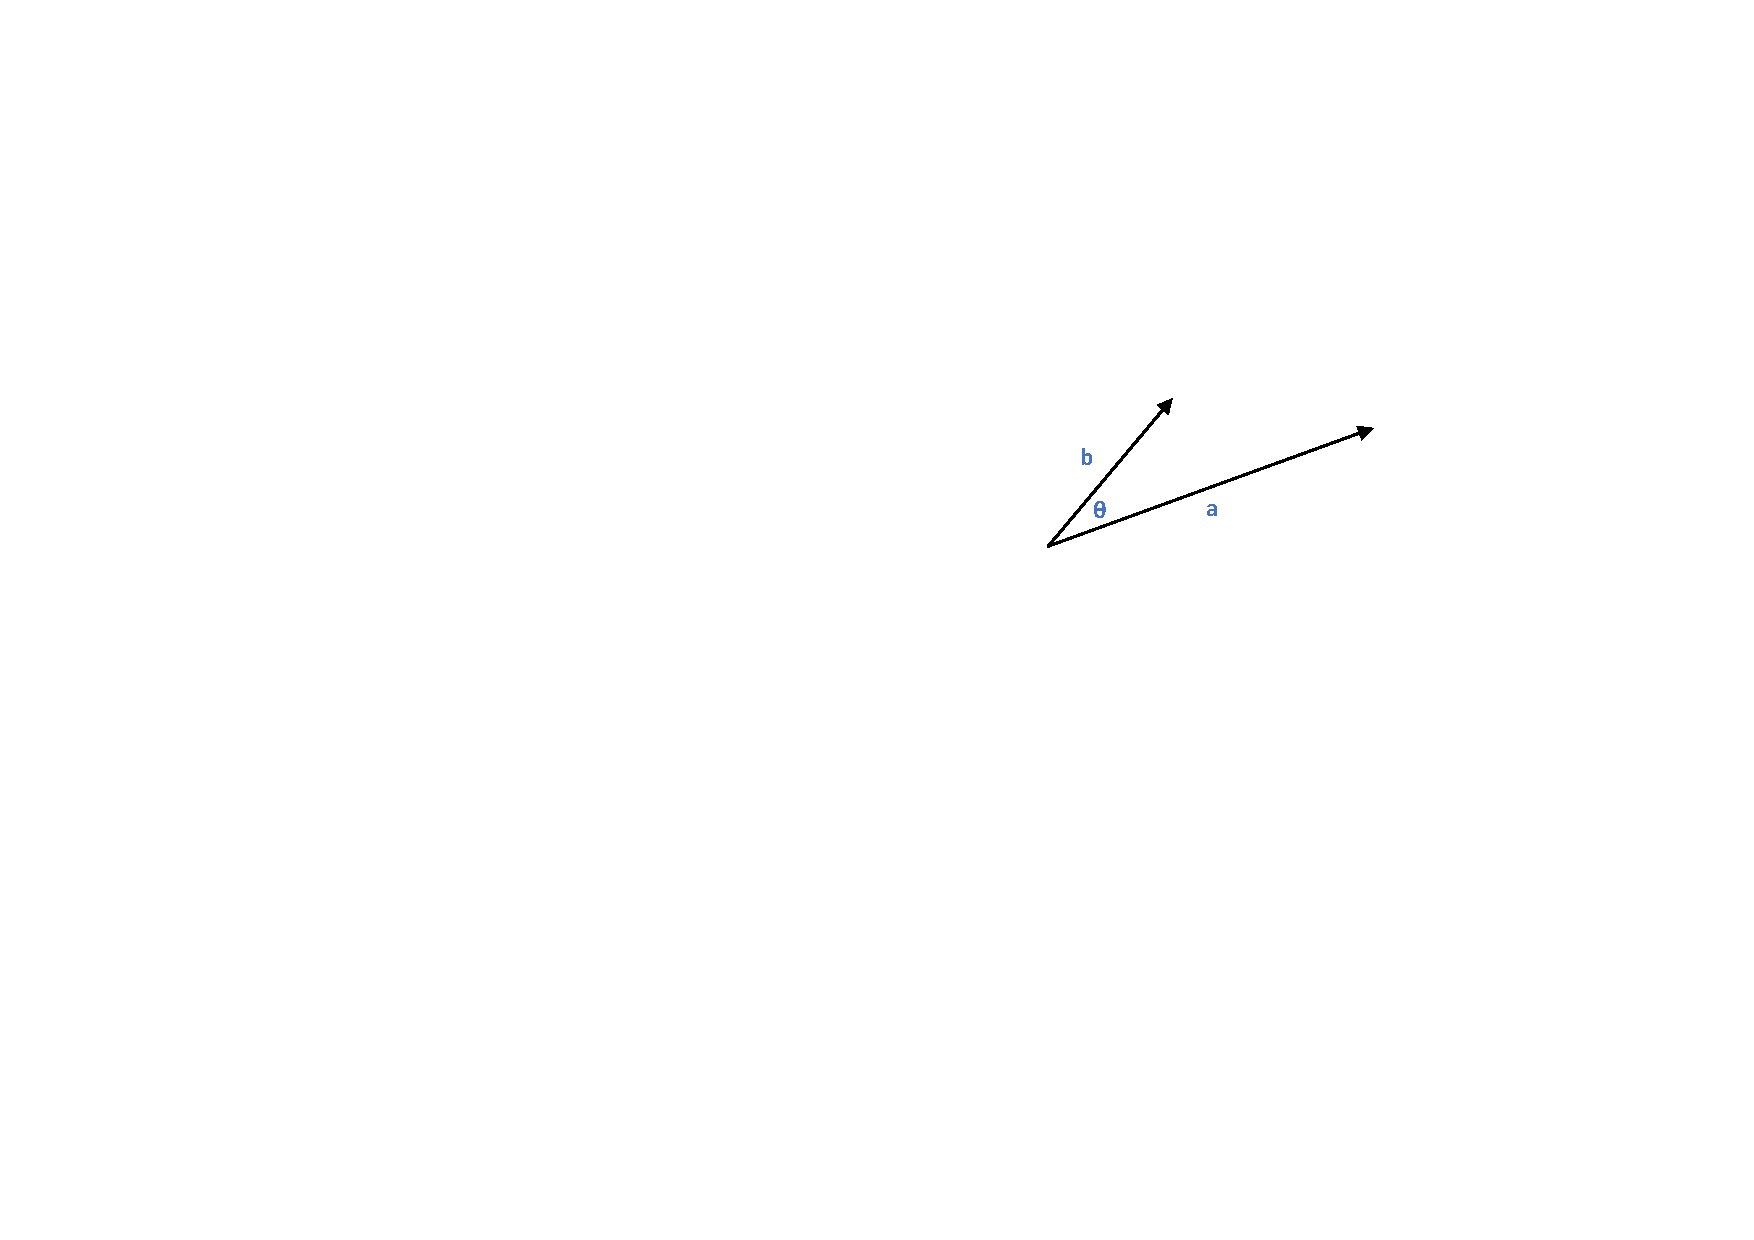
\includegraphics[scale=1]{DotProductDiagram.pdf}
    \caption{The dot product $\mathbf{a} \cdot \mathbf{b}$ can be calculated by the formula $|\mathbf{a}||\mathbf{b}| \cos{\theta}$.}
    \label{fig:DotProductDiagram}
\end{figure}

From here we can easily back calculate the angle between the vectors by solving the definition,

\begin{align*}
|\mathbf{a}||\mathbf{b}| \cos{\theta} &= \mathbf{a} \cdot \mathbf{b} \\
\cos{\theta} &= \frac{\mathbf{a} \cdot \mathbf{b}}{|\mathbf{a}||\mathbf{b}|} \\
\theta &= \arccos{\left(\frac{\mathbf{a} \cdot \mathbf{b}}{|\mathbf{a}||\mathbf{b}|}\right)}
\end{align*}

From this definition we can gain some more information about the CubeSat orientation in space. When the angle between the face of the cube and the flux vector is $0^{\circ}$ then the flux is at its maximum.

\begin{align*}
    \max{(\Phi_{\text{North, x}})} &= A |\mathbf{\Phi}_{\text{Sun}}(x, y, z)| \\
    \Phi_{\text{North, x}} &= -A \mathbf{\Phi}_{\text{Sun}}(x, y, z) \cdot \mathbf{\hat{n}}_{\textrm{North, x}}
\end{align*}

Therefore an angle can be determined for each face by doing,

\begin{align*}
    \theta = \arccos{\left( \frac{\Phi_{\text{North, x}}}{\max{(\Phi_{\text{North, x}})}} \right)}
\end{align*}

As shown in Figure \ref{fig:VectorNormaltoPlaneDiagram}.

\begin{figure}[H]
	\centering
	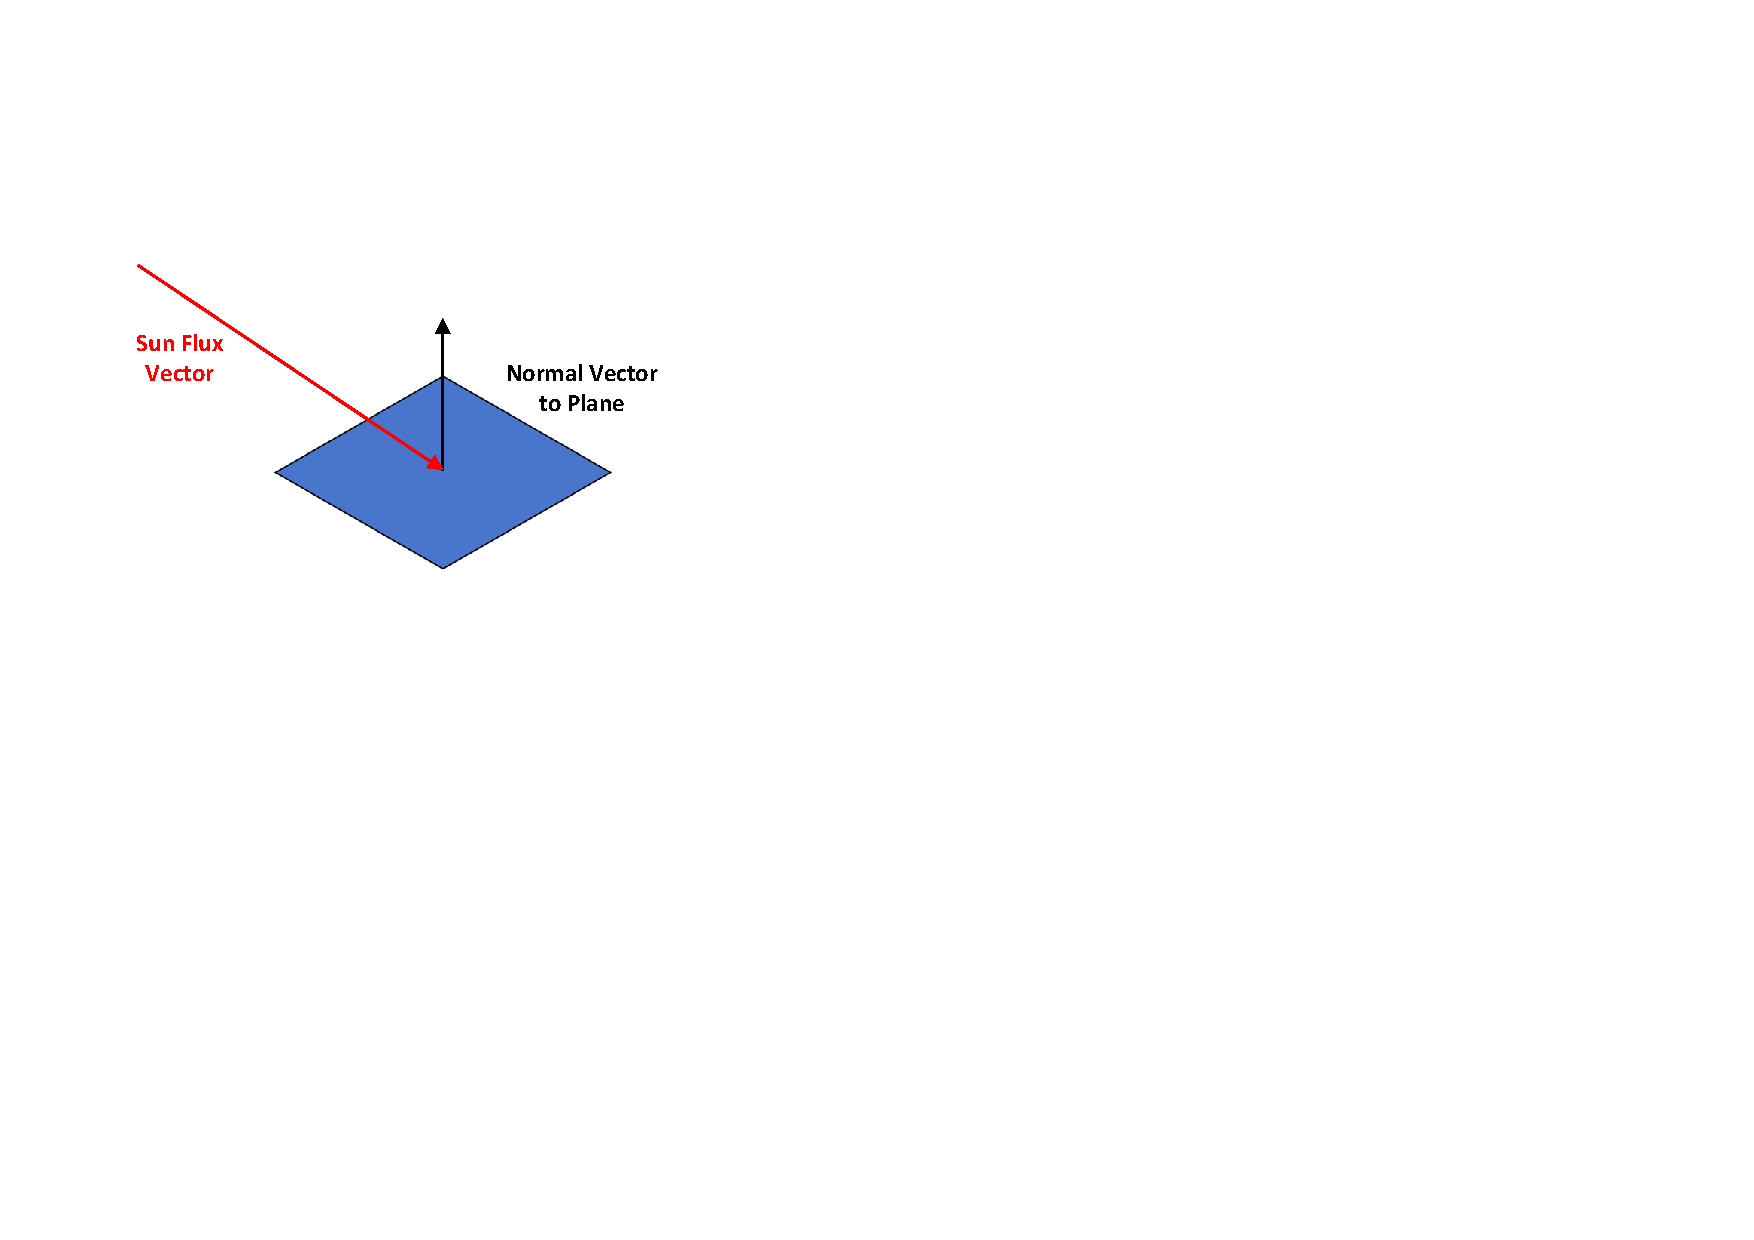
\includegraphics[scale=1]{VectorNormaltoPlaneDiagram.pdf}
    \caption{Sun flux vector hitting the plane of the cube face.}
    \label{fig:VectorNormaltoPlaneDiagram}
\end{figure}

When computing this however we find the angle is unique to the orientation of the cube (as far as we can tell). We have not sufficiently developed the technique enough to convert the angle back to roll, pitch and yaw angles.

Here is a sample printout of our MATLAB code in the \texttt{CubeDisplay.m} code.

\begin{verbatim}
SUN FLUX VECTOR
    SunFluxX: -1
    SunFluxY: 2
    SunFluxZ: 3

CURRENT CUBE ORIENTATION
    Roll: 0
    Pitch: 0
    Yaw: 0

LIGHT FLUX RECEIVED AT EACH CUBE FACE
(NEGATIVE VALUES HERE ARE PRESENTED FOR DIAGNOSTIC PURPOSES)
    NorthX: 4
    NorthY: -8
    NorthZ: -12
    SouthX: -4
    SouthY: 8
    SouthZ: 12

COMPUTE ANGLES FROM CUBE FACE TO FLUX VECTOR
    NorthX: 74.498640433063002
    NorthY: 1.223115332374239e+02
    NorthZ: 1.433007747995101e+02
    SouthX: 1.055013595669370e+02
    SouthY: 57.688466762576155
    SouthZ: 36.699225200489877
\end{verbatim}

And for when we perturb the roll orientation by 10 degrees we get,

\begin{verbatim}
SUN FLUX VECTOR
    SunFluxX: -1
    SunFluxY: 2
    SunFluxZ: 3

CURRENT CUBE ORIENTATION
    Roll: 10
    Pitch: 0
    Yaw: 0

LIGHT FLUX RECEIVED AT EACH CUBE FACE
(NEGATIVE VALUES HERE ARE PRESENTED FOR DIAGNOSTIC PURPOSES)
    NorthX: 4
    NorthY: -9.962240156100828
    NorthZ: -10.428507614811053
    SouthX: -4
    SouthY: 9.962240156100828
    SouthZ: 10.428507614811053

COMPUTE ANGLES FROM CUBE FACE TO FLUX VECTOR
    NorthX: 74.498640433063002
    NorthY: 1.317306884224274e+02
    NorthZ: 1.341695479077966e+02
    SouthX: 1.055013595669370e+02
    SouthY: 48.269311577572573
    SouthZ: 45.830452092203451
\end{verbatim}

Currently due to the time constraints on this project, we have been unable to derive a fundamental relationship between the roll, pitch and yaw angles and the angles calculated by the \texttt{CubeDisplay.m} script. This will be an area of further work, however it seems plausible to find the roll, pitch and yaw given this information.

For a simpler flux vector and roll/pitch/yaw perturbation the results are much easier to interpret. An example with a flux vector of $\langle 1, 0, 0 \rangle$ is shown below as well when pertubing the yaw angle by $10^{\circ}$. We can clearly see the angle computed at \texttt{SouthX} corresponds to the correct yaw angle perturbation.

\begin{verbatim}
SUN FLUX VECTOR
    SunFluxX: 1
    SunFluxY: 0
    SunFluxZ: 0

CURRENT CUBE ORIENTATION
     Roll: 0
    Pitch: 0
      Yaw: 10

LIGHT FLUX RECEIVED AT EACH CUBE FACE
(NEGATIVE VALUES HERE ARE PRESENTED FOR DIAGNOSTIC PURPOSES)
    NorthX: -3.939231012048832
    NorthY: 0.694592710667721
    NorthZ: 0
    SouthX: 3.939231012048832
    SouthY: -0.694592710667721
    SouthZ: 0

COMPUTE ANGLES FROM CUBE FACE TO FLUX VECTOR
    NorthX: 1.700000000000000e+02
    NorthY: 80
    NorthZ: 90
    SouthX: 10.000000000000012
    SouthY: 9.999999999999999e+01
    SouthZ: 90
\end{verbatim}


In reality the negative flux numbers would also be zero. This would help narrow down the possible solutions by providing us information about what octant the cube is oriented to. A more rigorous look at the angle information may yield a numerical solution to the problem of determining yaw, pitch and roll. However as of now, we have been unable to find that solution.

\subsection{Code Results}

Our code is fully capable of simulating the diode responses for each cube face given a known flux vector and a specified roll, pitch and yaw orientation.

A more rigorous treatment of the interpretation of the angles between the known flux vector and the cube faces however is required to properly back calculate the roll, pitch and yaw orientation. Currently this is beyond our capabilities, however this research should serve as a good starting point for future iterations of this project.

We have generated a code base for this project and posted it as a publicly available repository on GitHub. It can be found here \url{https://github.com/saribeiro/CubeSatOrientation.git}

\section{Future Improvements}

\subsection{Problems with Roll, Pitch and Yaw}

Regarding the representation of rotations or the linear combination of rotations, it is easy to understand and use the roll, pitch and yaw matrices. However it is known that certain issues arise with using this relatively simplistic method of representing rotations in space.

The issue of `gimbal lock' often arises in attitude control systems that only use roll, pitch and yaw where a degree of freedom is lost due to two parameters lining up. This can result in a complete loss of orientation and the inability to regain control of the spacecraft. One such mathematical representation that helps avoid ambiguous rotations or gimbal lock from occurring is the quaternion representation for rotations.

Perhaps if we rebuilt our mathematical model using quaternion algebra to represent the rotations and to calculate the light fluxes on each cube face, it may yield solvable equations that can pinpoint orientations exactly.

\subsection{Quaternions}

Quaternions are a mathematical object invented by Sir William Rowan Hamilton that is an extension of the complex numbers $\mathbb{C}$. Quaternions are sometimes referred to as `hypercomplex numbers' and are symbolized by the set $\mathbb{H}$. Quaternions have four components associated with them.

A quaternion $\mathbf{q}$ can be written as follows,

\begin{equation*}
    \mathbf{q} = q_{0} + q_{1} \cdot \mathbf{i} + q_{2} \cdot \mathbf{j} + q_{3} \cdot \mathbf{k}
\end{equation*}

There are four `unit vectors' associated with quaternions. We have the scalar value 1, and the other three components $\mathbf{i}$, $\mathbf{j}$, $\mathbf{k}$. Quaternion algebra does not preserve the commutative property and thus the multiplication rules for quaternions are slightly more complicated. Figure \ref{fig:QuaternionChart} shows how the multiplication of unit quaternions works. As you can see multiplication is not commutative.

\begin{figure}[H]
	\centering
	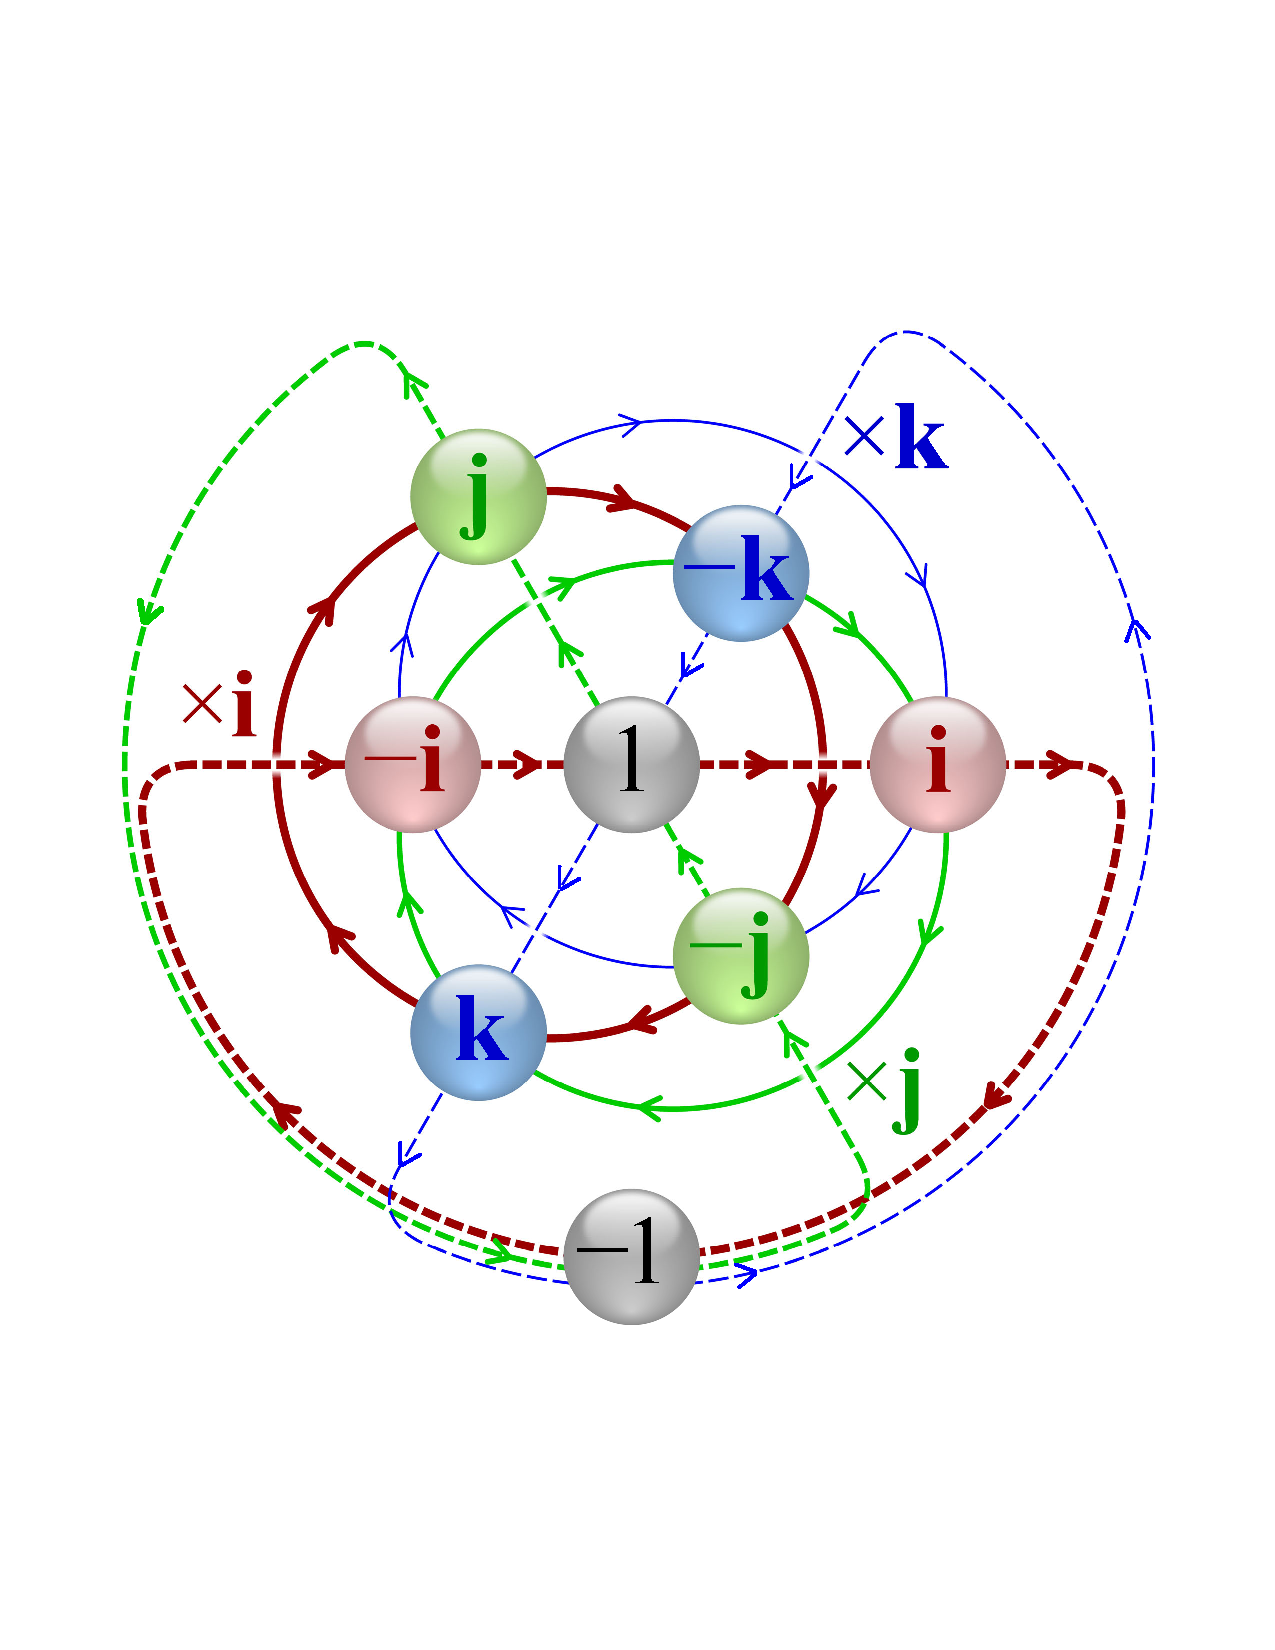
\includegraphics[scale=0.6]{CayleyQ8_QuaternionMultiplicationChart.pdf}
    \caption{Descriptive chart to show how quaternion multiplication works. }
    \label{fig:QuaternionChart}
\end{figure}

\begin{center}
    \begin{tabular}{|c|cccc|}
    \hline
        $\times$ & 1 & i & j & k \\ \hline
        1 & 1 & i & j & k \\
        i & i & -1 & k & -j \\
        j & j & -k & -1 & i \\
        k & k & j & -i & -1 \\ \hline
    \end{tabular}
\end{center}

William Hamilton's original motivation for developing quaternions was to extend the rotation properties of complex numbers to three dimensions. Ordinarily complex numbers are able to encode rotations on a two dimensional plane as a single complex number with a real and imaginary component.

MATLAB has a large number of quaternion capabilities built into it. We have compiled some sample code in MATLAB for working with quaternions.

\subsection{Rotation Using Quaternions}

Quaternion rotation can be achieved by specifying an axis about which we rotate our point(s) (described as a unit vector $\langle r_{x}, r_{y}, r_{z} \rangle$) and the rotation angle by which we want to rotate by.

Once we have built our rotation quaternion (symbolized by $\mathbf{q}_{\theta}$) we can rotate our three dimensional point described as a vector $\mathbf{r}$ by the following computation,

\begin{equation*}
    \mathbf{r}_{\text{rotated}} = \mathbf{q} \mathbf{r} \mathbf{q^{*}}
\end{equation*}

The quaternion conjugate $\mathbf{q}^{*}$ is identical to the idea of a complex conjugate. If the quaternion $\mathbf{q} = q_{0} + q_{1} \cdot \mathbf{i} + q_{2} \cdot \mathbf{j} + q_{3} \cdot \mathbf{k}$, then the conjugate is $\mathbf{q}^{*} = q_{0} - q_{1} \cdot \mathbf{i} - q_{2} \cdot \mathbf{j} - q_{3} \cdot \mathbf{k}$. The vector $\mathbf{r}$ can be thought of a quaternion where the first scalar argument is simply zero. Thankfully the associative property applies to quaternion algebra.

Calculating the rotation quaternion is actually quite trivial and it looks awfully similar to Euler's formula which represents complex number rotations.

\begin{align*}
    \mathbf{q}_{\theta} &= \cos{\left(\frac{\theta}{2}\right)} + (r_{1} \cdot \mathbf{i} + r_{2} \cdot \mathbf{j} + r_{3} \cdot \mathbf{k}) \cdot \sin{\left(\frac{\theta}{2}\right)} \\
    \mathbf{q}_{\theta} &= \cos{\left(\frac{\theta}{2}\right)} + \mathbf{r} \cdot \sin{\left(\frac{\theta}{2}\right)}
\end{align*}

Below is an example of using MATLAB's built in quaternion libraries and capabilities to rotate a cube about a defined axis. The full code for this is included in the appendix of this paper. See the results below in Figures \ref{fig:Quaternion_OriginalCube} and \ref{fig:Quaternion_RotatedCube}. The rotation was computed by this code snippet,

\setstretch{1}
\lstinputlisting[firstnumber=96, firstline=96, lastline=103]{Quaternions.m}
\setstretch{\docstretch}

\begin{figure}[H]
	\centering
	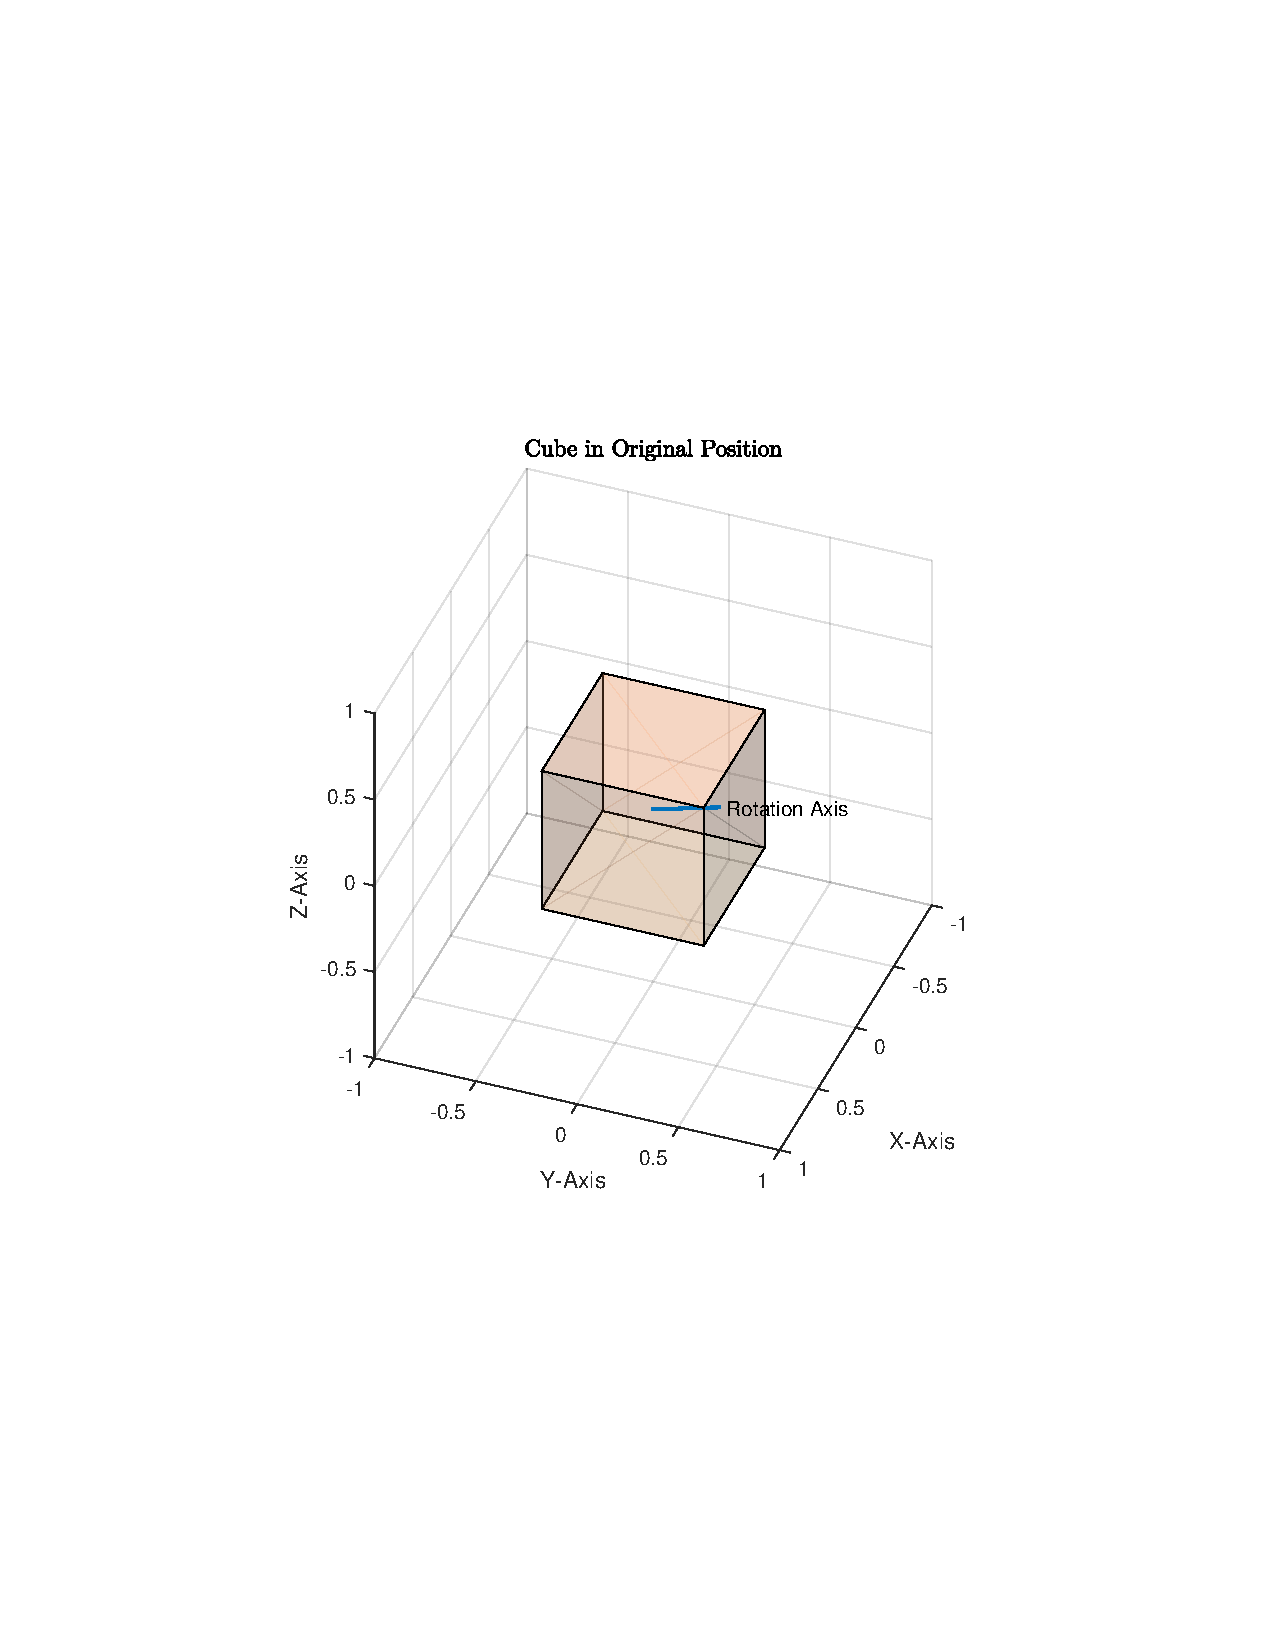
\includegraphics[scale=0.8]{Quaternion_OriginalCube.pdf}
    \caption{Original cube orientation. Rotation axis is shown as a blue unit vector along the vector $\langle 1, 1, 1 \rangle$.}
    \label{fig:Quaternion_OriginalCube}
\end{figure}

\begin{figure}[H]
	\centering
	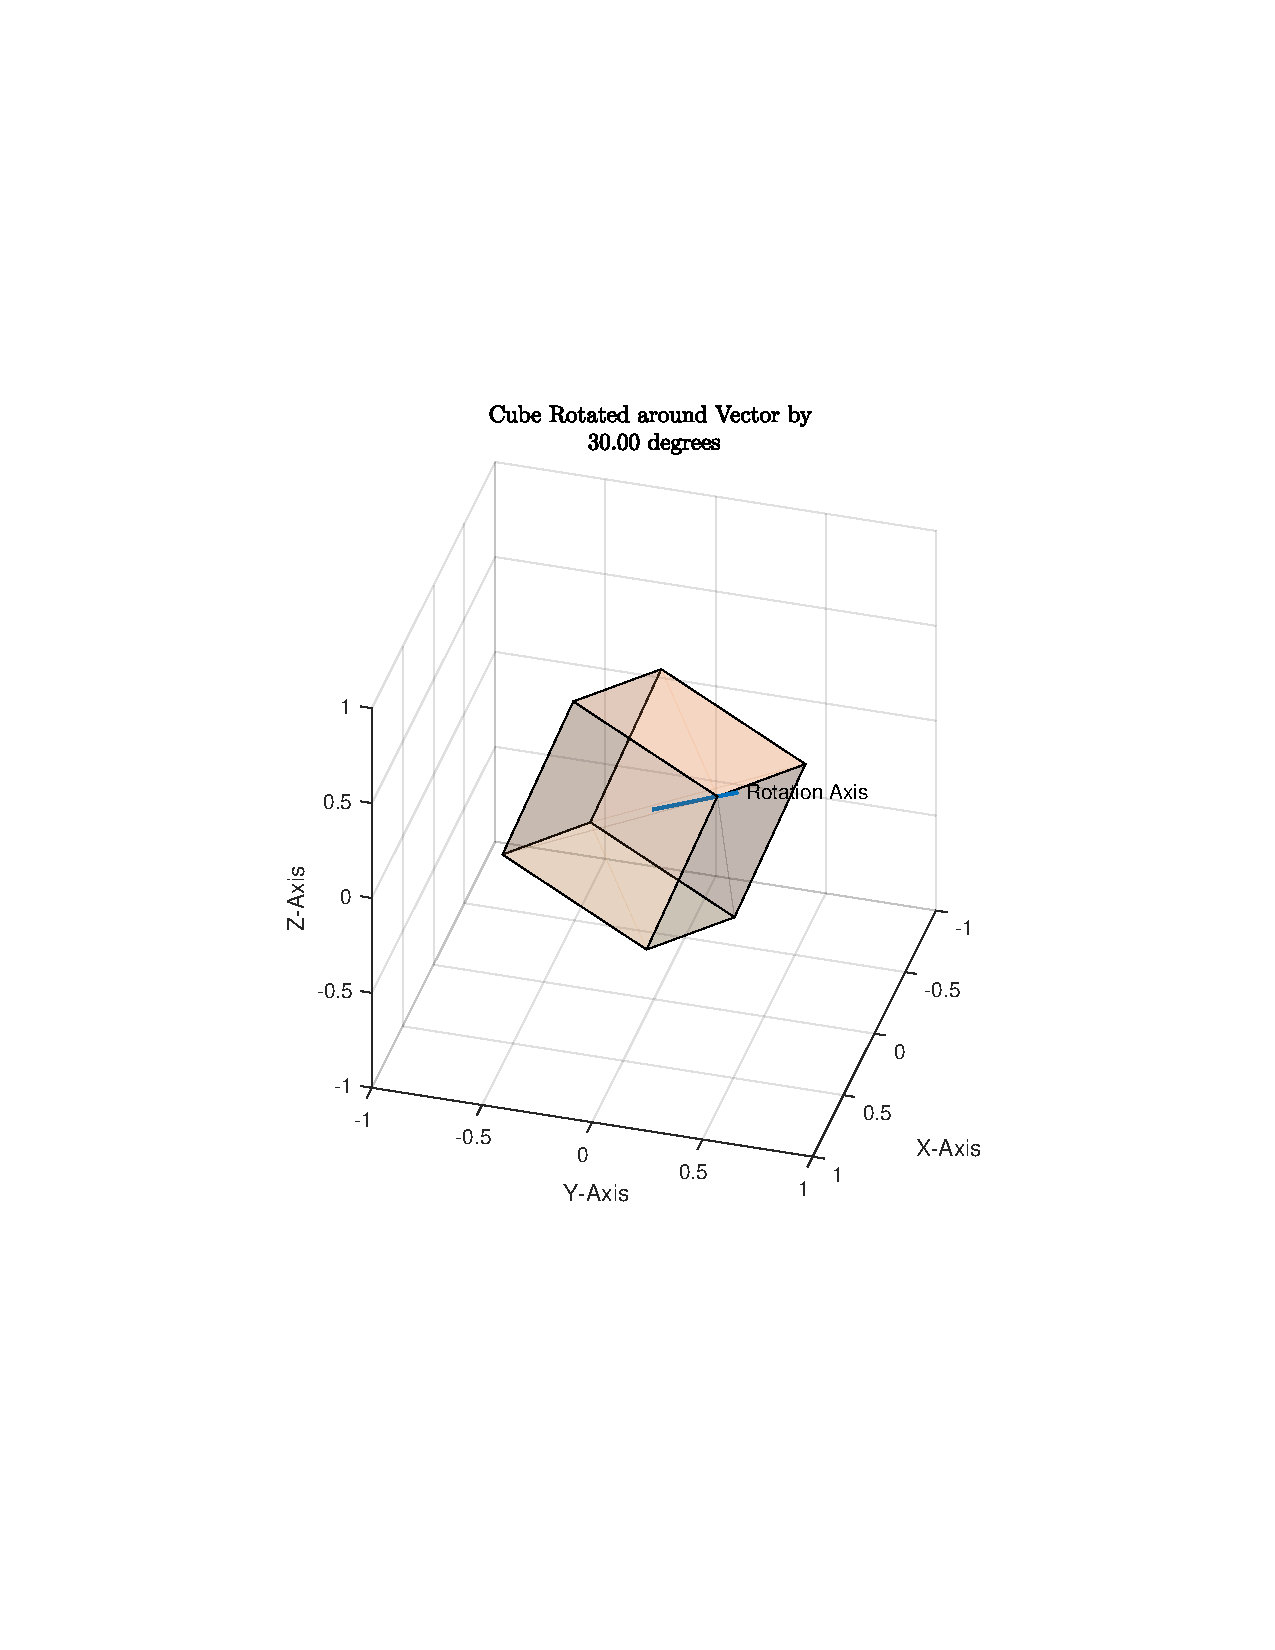
\includegraphics[scale=0.8]{Quaternion_RotatedCube.pdf}
    \caption{Cube has been rotated by $30^{\circ}$ about the rotation axis.}
    \label{fig:Quaternion_RotatedCube}
\end{figure}

\section{Concluding Remarks}

A more rigorous treatment of the interpretation of the angles between the known flux vector and the cube faces however is required to properly back calculate the roll, pitch and yaw orientation. Currently this is beyond our capabilities, however this research should serve as a good starting point for future iterations of this project.

We have generated a code base for this project and posted it as a publicly available repository on GitHub. It can be found here \url{https://github.com/saribeiro/CubeSatOrientation.git}. Future iterations of this project may find it far easier to rebuild or build upon our model using quaternion algebra and quaternion methods to describe cube rotations and cube orientations.


\newpage
\section{MATLAB Code}

\subsection{Cube Display Code}

The purpose of this MATLAB code is to generate a useful visual representation of the item we are talking about and to generate useful figures and test data to spot check our assumptions.

\setstretch{1}
\lstinputlisting{CubeDisplay.m}
\setstretch{\docstretch}
\newpage

\subsection{Diode Response Code}

The purpose of this MATLAB code is to simulate the photo-diode responses given a sun vector, a starting orientation (roll, pitch and yaw) and stepping the degrees of one parameter (roll, pitch or yaw). The resulting data is parsed into a CSV file for later examination.

\setstretch{1}
\lstinputlisting{ComputeDiodeResponse.m}
\setstretch{\docstretch}
\newpage


\subsection{Quaternion Code for Future Work}

The purpose of this MATLAB code is to demonstrate the rotational capabilities using quaternions for future development. Perhaps in the next iteration of this project, we will build our model based solely on quaternion algebra.

\setstretch{1}
\lstinputlisting{Quaternions.m}
\setstretch{\docstretch}
\newpage

\end{document}
